%% ----------------------------------------------------------------------------
% BIWI SA/MA thesis template
%
% Created 09/29/2006 by Andreas Ess
% Extended 13/02/2009 by Jan Lesniak - jlesniak@vision.ee.ethz.ch
%% ----------------------------------------------------------------------------
\newpage
\chapter{Training CNNs using fully annotated segmentation masks}
Nowadays, the CNNs have evolved with great speed to solve major problems in classical computer vision scenario. Instead of using classical image processing filters, the CNNs are specialized to learn feature maps from the examples provided and, specific to the task at hand. The resereach in CNNs has evolved to provide an end-to-end solution without any requirement of pre/post-processing of images. Thus, the state-of-the-art approach to solve any task in computer vision is to use CNNs. In this chapter, we describe the diffculties faced in using the CNN for our task and the alternate approach we took to overcome the limitations and difficulties.

\section{Overview}
The classical way to use the CNNs is to design a neural network architecture and train it from scratch. One of the challenge in this classical approach is the choice of architecture of network and choice of training parameters such as initialization, loss function etc. In literature, we can find different architectures of neural networks specially designed for the task of segmentation, one of the popular architecture is U-Net \cite{unet}. The major prerequisite of this approach to perform well is huge amount of training data: images and ground truth labelled data. For classical problems such as segmenting faces etc., a huge amount of images available on internet can used to generate a training dataset. This becomes a problem in the medical domain where it is very costly to generate images and, even more costly and time-consuming to prepare it for training. Although, due to advancement in technology, the microscopic images can be generated with an ease and is not a time-consuming and tedious process anymore. For example, the microscopic images of liver tissue were generated automatically with the help of a robotic arm. But, the diffuclty in using such CNNs lies with generating significant amount of annotated data for training. For our problem of image segmentation, we described the problem faced by experts and doctors in generating fully annotated segmented masks in introduction. This poses a limitation in using such CNNs for our task of segmentation of objects in microscopics images. The alternate approach to train CNNs in such cases has been by use of transfer learning.

\section{Transfer Learning}
The use of transfer learning provides a way to compensate for the scarce training data.
Transfer learning tries to store the knowledge gained from solving one problem and applying it to a different but related problem. Thus, in practice, it is becoming rare to train an entire CNN from scratch, as it is relatively difficult to have a dataset (images and labels) of sufficient size for training. Instead, one of the common way to perform transfer learning is to use a pre-trained network, either to initialize a network or to extract required feature maps. Shelmar et al. \cite{long:2014} designed a "fully convolutional" network that takes input of arbitrary size and produces segmented output for a complete image. They adapted contemporary classification networks (AlexNet, the VGG net, and GoogLeNet) into fully convolutional networks and transfer their learned representations by fine-tuning to the segmentation task. Similar to Shelmar, we could have chosen one of the contemporary classification networks and fine-tuned them for segmenting objects in liver tissue images. But, due to having very small set of slices for training (10 slices with fully annotated ground truth masks), we decided to choose a network pre-trained and modified for task of image segmentation. Then we could be able to fine-tune it for our task even with such small amount of images. Recently, Caelles et al. \cite{osvos} described an architecture using a pre-trained model which performed well for the task of \textbf{semi-supervised} video object segmentation. This paper termed the network designed as \textbf{OSVOS} i.e. One shot video object segmentation.



\section{One shot Video object segmentation (OSVOS)}
Caelles et al. \cite{osvos} implemented an architecture to segment an object in a video sequence using only one frame for training. The network is trained to learn object semantics from only one frame and generate segmentation mask for remaining all frames. The segmentation works well if the object remains in relatively similar shape and size. 
The example result of this architecture can be seen in figure 2.1.
\begin{figure}[h!]\label{fig:osvos1}
\centering
 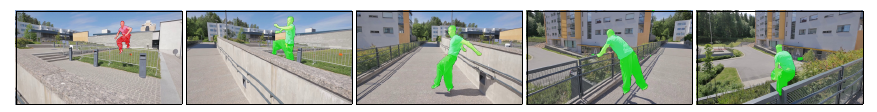
\includegraphics[width=1.0\linewidth]{figures/osvos1.png} 
\caption{ Example result of OSVOS \cite{osvos}: The segmentation of the first frame (red) is used to learn semantics of interested object, whicich is segmented in the rest of the frames independently (green).}
\end{figure}

Caelles et al. \cite{osvos} modified a CNN network pre-trained for image recognition and fine-tuned it for object segementation, as shown in figure 2.2. This was achieved by training it on a set of videos with manually annotated objects. They designed OSVOS by adopting a fully convolutional network (FCN), suitable for dense predictions. The major drawback with use of FCN for task of segmentation is the coarse scale of the deeper layers due to downsampling of feature maps. This leads to inaccurately localized predictions. One way to overcome this drawback is by making use of skip connections of initial larger feature maps \cite{unet}. To avoid this inaccuracy, OSVOS combined information from all network layers to predict segmentation mask for the image. \par

\begin{figure}[h!]\label{fig:osvos1}
\centering
 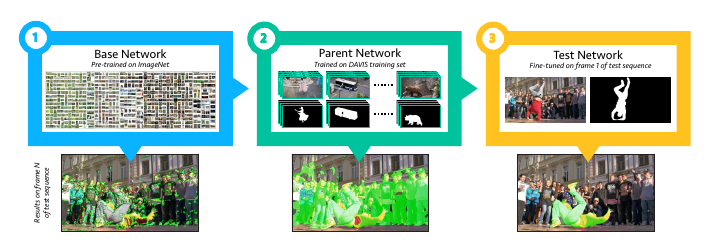
\includegraphics[width=1.0\linewidth]{figures/osvos_train.png} 
\caption{Overview of OSVOS \cite{osvos}: (1) Pre-trained base CNN; its results in terms of segmen-
tation. (2) Training of network for task of object segmentation, parent network. (3) By fine-tuning on a segmentation example for the specific object in first frame, the network rapidly adopts to focus on that target.
}
\end{figure}

 The design of architecture of OSVOS network drew inspiration from the CNN architecture of \cite{maninis:2016}, originally used for biomedical image segmentation of retinal vessles. The OSVOS network was based on the pre-trained VGG \cite{vgg} network. They removed the last fully connected layers and the output from the deeper layers was interpolated to orginal image size. The VGG architecture can be divied into 5 stages, each consisting of groups of convolutional plus Rectified Linear Units (ReLU). Between these  5 stages, pooling operations downscale the feature maps as we go deeper into the network. The output feature maps (before pooling) from stage 2 to 5 are connected using convolutional layer to form separate skip paths. The output feature maps from each skip path are fused linearly and upscaled as required to generate a segmentation mask of same size of original image. They call these masks as "side outputs". In addition, the feature maps from separate paths are are concatenated to construct a volume with information from different levels of layers. Finally, they linearly fuse the volume of feature maps to a single output, called "main output", which has the same dimensions as the image. They computed cross entropy loss using both "main" and "side" outputs. The use of information from all layers enables the network not to loose finer details of the image.



\section{Motivation for using OSVOS}
Once the base network has been modified and trained to perform object segmentation, the parent network can be considered as a pre-trained network for image segmentation. The network is able to learn object semantics and identify various objects in the image. The test network, as shown in figure 2.2, only needs information about object of interest and starts considering rest of image as background. The test network learns about object from a single frame i.e. a single image and generates segmentation mask for all other frames independently. If we consider the 3D volume of slices of liver tissue similar to a video, each slice can be thought of as a frame. Motivated by this similarity, we decided to fine-tune the parent network using few slices and generate the segmentation mask for the whole 3D volume. The liver vesicles in different slices of 3D volume are approximately similar in size and shape, and thus, fine-tuning using few slices can enable the network to learn various features of vesicles. The use of OSVOS fits our problem due to limited availablity of training data. 

\section{Experiment and results}
We annotated liver vesicles of different size and shapes in few randomly chosen slices. These slices were used to fine-tune the parent OSVOS network to target the object of interest. In literature, we can find that network tends to overfit on a relatively small dataset. The use of augmentation helps in generating more data and avoids network from overfitting. We generated more data using cropped and flipped slices for fine-tuning. The segmentation output from CNN trained using 2 slices is also shown in figure 2.1. It can be seen that the OSVOS is able to learn about the features of object and generates a good segmentation mask with accuracy (F-score) of 0.86.\par

\begin{figure}[h!]\label{fig:cnnslices}
\centering
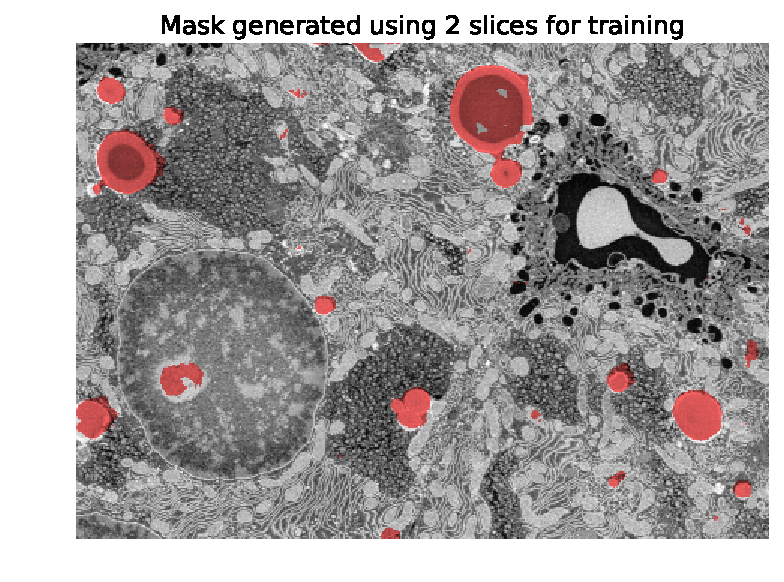
\includegraphics[width=0.9\linewidth]{figures/cnn_mask_2slice.pdf} \\
\caption{Predicted segmentaion mask for part of slice 45}
\end{figure}

In this thesis, we are more interested in observing variation in accuracy with the increase in amount of training data. Thus, we tested OSVOS by fine-tuning it using different number of slices, staring from 1 slice and increasing to 10 slices. For our experiment, set of slice with number \{1,7,10,18,24,52,62,72,80,88\} were used for training. While training, the batch size was always 1. In case of multiple slices i.e. more than 1 slice for training, each slice was fed as separate input to train the network. The set of slices chosen was in ascending order of their number i.e. for training with 3 slices, slice no. \{1,7,10\} were used and for training with 4 slices, slice no. \{1,7,10,18\} were used. These slices were fed to network as an independent image in random order. Once, the parent network was fine-tuned, the test network predicted results for test set. We were not able to test the network on whole 3D volume due to lack of availability of ground truth segmentation mask for whole volume. The test set consisted of part of image from slice number 15, 30 and 45. We had multiple masks annotated by experts for these slices. Even for a single slice, for example 15, we had multiple mask differing from each other annotated by same expert. We generated a reference mask using STAPLE algorithm and computed segmentation accuracy for test slices using these refernce masks. The result of the change in traing data can be seen in figure 2.4.

\begin{figure}[h!]\label{fig:cnnslices1}
\centering
 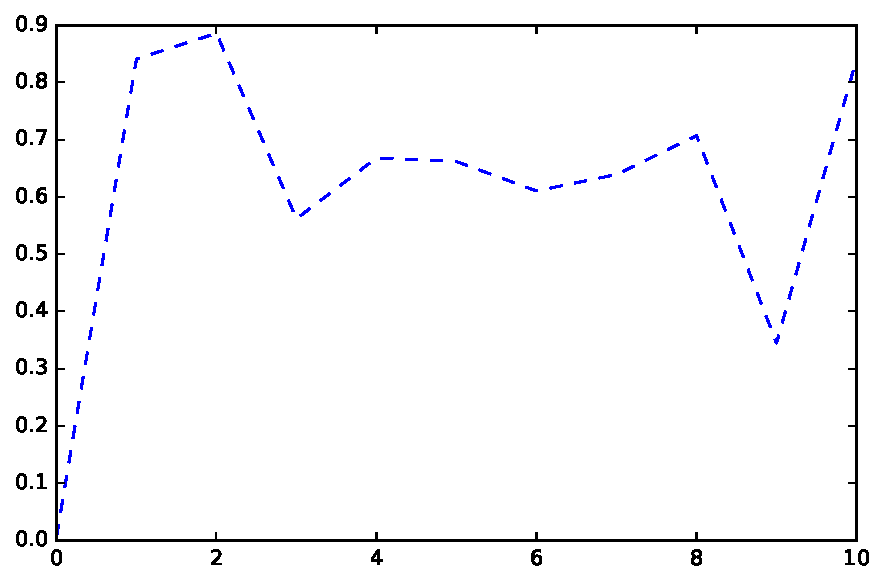
\includegraphics[width=0.9\linewidth]{figures/cnn_diff_slices.pdf} 
\caption{Segmentation accuracy for different amount of training data (Number of slices)}
\end{figure}

We expected an increase in performance with the increase in the amount of training data. This does not happen as CNN is not able to converge equivalently for all cases. We see a significant drop after addition of $9^{th}$ slice, i.e. slice number 80. On analysis, we realized that the training with each slice independently in each forward pass is not allowing the network converge easily with increase in number of slices. Instead, the better way would be to use all available slices in a batch to train the network. Although, we were able to get a significant accuracy with such few annotated slices but it is important to remember here that annotating one slice is not same as annotating one object in a video. We can observe that a single slice contains multiple objects, as shown in figure 2.3. Also, if the experts make few changes in annotated masks used for training, this will force us to train the network again. These difficulties motivated us to try semi-supervised learning using RF for our task of segmentation and try to achieve similar accuracy.

